\documentclass[a4paper,12pt]{book} % nie: report!


\usepackage[T1,plmath]{polski} % lepiej to zamiast babel!
\usepackage[utf8]{inputenc} % w razie kłopotów spróbować: \usepackage[utf8x]{inputenc}
\usepackage{fancyhdr} % nagłówki i stopki
\usepackage{indentfirst} % WAŻNE, MA BYĆ!
\usepackage[pdftex]{graphicx} % to do wstawiania rysunków
\usepackage{amsfonts} % pakiety od AMS, ułatwiają składanie pewnych techniczno-matematcyznych rzeczy
\usepackage{amsmath} % to do dodatkowych symboli, przydatne
\usepackage{amssymb} % to też do dodatkowych symboli, też przydatne
\usepackage{amsthm}
\usepackage[pdftex,
            left=1.1in,right=1.1in,
            top=1.1in,bottom=1.1in]{geometry} % marginesy
\usepackage{float}

\usepackage[font=small,labelfont=bf]{caption}
\usepackage{cite}

\usepackage{siunitx}

\usepackage[colorlinks=true]{hyperref} % odnośniki interaktywne w PDFie
\hypersetup{allcolors=black} % odnośniki proszę zostawić kolorowe -- a jeśli ktoś nie lubi to zmienić na czarne dopiero w ostatniej wersji!
\usepackage{listings}
\lstset{
    basicstyle=\footnotesize\tt,
    numbers=left,
    numberstyle=\tiny,
    frame=tb,
    tabsize=4,
    columns=fixed,
    showstringspaces=false,
    showtabs=false,
    keepspaces,
    captionpos=t,    
    commentstyle=\color{red},
    keywordstyle=\color{blue}
}
\newfloat{lstfloat}{htbp}{lolst}[chapter]
\floatname{lstfloat}{Listing}
\def\lstfloatautorefname{Listing}

\usepackage{booktabs}

\usepackage{bytefield}

\usepackage{./styles/listings-rust}

% \usepackage{cascadia-code}

% jesli potrzeba, można oczywiście wstawić inne pakiety i swoje definicje...

\newcommand{\translation}[1]{(ang. \textit{#1})}
% \newcommand{\isqrc}{$I^2C$}
\newcommand{\isqrc}{I\textsuperscript{2}C}
\DeclareSIUnit{\kilobitpersecond}{kbps}

% definicje nagłówków i stopek
\pagestyle{fancy}
\renewcommand{\chaptermark}[1]{\markboth{#1}{}}
\renewcommand{\sectionmark}[1]{\markright{\thesection\ #1}}
\fancyhf{}
\fancyhead[LE,RO]{\footnotesize\bfseries\thepage}
\fancyhead[LO]{\footnotesize\rightmark}
\fancyhead[RE]{\footnotesize\leftmark}
\renewcommand{\headrulewidth}{0.5pt}
\renewcommand{\footrulewidth}{0pt}
\addtolength{\headheight}{1.5pt}
\fancypagestyle{plain}{\fancyhead{}\cfoot{\footnotesize\bfseries\thepage}\renewcommand{\headrulewidth}{0pt}}


% interlinia
\linespread{1.25}

\bibliographystyle{plainurl}

\begin{document}

\include{src/title_page}

\sloppy

\thispagestyle{empty}

\newpage{}



\thispagestyle{empty}

\newpage{}



\tableofcontents{}

\chapter*{Wstęp} % z gwiazdką, więc bez numerka...
\addcontentsline{toc}{chapter}{Wstęp} % ...ale w spisie treści ma być...
\chaptermark{Wstęp} % ...i w paginie górnej

Rozwój technologii cyfrowych oraz rosnąca automatyzacja procesów
przemysłowych i~domowych sprawiają, że dokładny i~ciągły pomiar
parametrów środowiskowych staje się coraz istotniejszym elementem
współczesnej inżynierii. Dostępne na rynku konsumenckim stacje pogodowe,
mimo rosnącej funkcjonalności, charakteryzują się ograniczoną dokładnością
pomiarową oraz koniecznością zasilania z~sieci elektrycznej lub okresowej
wymiany baterii jednorazowych, co w~przypadku montażu zewnętrznego,
w~miejscach trudno dostępnych lub oddalonych, jest niepraktyczne bądź
generuje dodatkowe koszty eksploatacyjne.
 
Celem niniejszej pracy jest zaprojektowanie i~wykonanie autorskiego
czujnika klimatycznego pozbawionego akumulatora, zasilanego wyłącznie
energią pochodzącą z~paneli fotowoltaicznych, magazynowaną
w~superkondensatorach. Zbudowane urządzenie dokonuje pomiaru temperatury,
wilgotności względnej, ciśnienia atmosferycznego, natężenia oświetlenia
oraz poziomu promieniowania jonizującego, a~zgromadzone dane przesyła
bezprzewodowo do stacji bazowej za pomocą autorskiego protokołu radiowego.
Realizacja projektu obejmowała zarówno zaprojektowanie i~wykonanie układu
elektronicznego, jak i~opracowanie oprogramowania sterującego
mikrokontrolerem ATmega328p, zaimplementowanego w~języku Rust, którego
mechanizmy bezpieczeństwa pamięci, weryfikowane statycznie na etapie
kompilacji, stanowią alternatywę dla tradycyjnie stosowanego w~systemach
wbudowanych języka C.
 
Praca składa się z~sześciu rozdziałów. Rozdziały pierwszy i~drugi mają
charakter wprowadzający --- omówiono w~nich dostępne na rynku moduły
pomiarowe, technologie magazynowania energii oraz porównanie języków
programowania stosowanych w~systemach wbudowanych. Rozdział trzeci
przedstawia założenia projektowe zrealizowanego urządzenia, rozdziały
czwarty i~piąty opisują odpowiednio jego warstwę sprzętową i~programową,
a~rozdział szósty przedstawia wyniki przeprowadzonych pomiarów.

\chapter{Wprowadzenie do tematyki}
\section{Czujniki klimatyczne}
Współczesny rozwój technologiczny w~połączeniu z~postępującymi
zamianami klimatu oraz rosnącą automatyzacją procesów 
przemysłowych i~urządzeń domowych sprawiły, że precyzyjne
obserwowanie i~dokumentowanie parametrów środowiskowych stało się
nieodłącznym elementem współczesnej inżynierii.

Głównym zadaniem czujników klimatycznych jest ciągła 
i~bezobsługowa akwizycja danych dotyczących parametrów atmosfery 
w~wybranym obszarze. Dane te są kluczowe w~wielu dziedzinach
życia gospodarczego i~społecznego. W~rolnictwie precyzyjnym
\translation{smart agriculture} pozwalają na optymalizację 
nawadniania i~ochrony upraw [TODO: citation needed], 
w~aglomeracjach miejskich służą do monitorowania smogu i~poziomu
zanieczyszczeń powietrza, natomiast w~systemach zarządzania 
budynkami \translation{Building Management Systems} stanowią 
podstawę sterowania procesami klimatyzacji, wentylacji 
i~ogrzewania.

[TODO: Może jeszcze jeden akapit? Praca Wołodko? Modularność?]

\section{Moduły pomiarowe}
Do podstawowych wielkości fizycznych rejestrowanych przez 
czujniki klimatyczne zalicza się przede wszystkim temperaturę, 
wilgotność względną oraz ciśnienie atmosferyczne. Do pomiaru tych 
wielkości coraz rzadziej wykorzystuje sie bezpośrednio połączone
z~układem czujniki analogowe, a~są one wypierane przez moduły 
integrujące elementy pomiarowe, dedykowane przetworniki
analogowo-cyfrowe (ADC, ang. \textit{analog-digital converter})
oraz fabryczne obwody kalibracyjne w~jednej obudowie. Pozwala to, 
między innymi, wyeliminować problem zakłóceń elektromagnetycznych 
indukowanych w~przewodach sygnałowych. Ponadto, projektanci modułów
implementują algorytmy linearyzacji charakterystyk sensorów
oraz filtry szumów analogowych po stronie samego modułu, pozwalając
na wygodniejszych odczyt danych.


\section{Zasilanie czujników}
[Panele słoneczne i magazyn energii]

\chapter{Programowanie systemów wbudowanych}
\section{Języki programowania}
[C, C++, Rust, MicroPython, co do jakiego mikrokontrolera]
\section{Obsługa magistrali}
[Opisz czym jest I2C z perspektywy kodu]

\chapter{Część sprzętowa}

\section{Założenia projektowe}
\subsection{Niski pobór mocy}
\subsection{Zastosowanie paneli fotowoltaicznych}
\subsection{Superkondesatory a akumulatory}
\subsection{Komunikacja radiowa}

\newpage{}

\section{Podstawowe elementy układu}

Schemat elektryczny, stworzony na potrzeby tej pracy, został podzielony na segmenty pełniące konkretne funkcje.

\subsection{Sekcja ładowania superkondesatorów}
Zastosowanie paneli fotowoltaicznych jako jedynego źródła energii do ładowania superkondensatorów wiąże się z określonymi ograniczeniami. Ze względu na zmienne warunki nasłonecznienia, wynikające z czynników zewnętrznych, takich jak okresowe zacienienie panelu przez elementy otoczenia lub zmiany pory dnia, napięcie generowane na wyjściu panelu fotowoltaicznego nie ma charakteru stałego. W celu zapobieżenia wystąpieniu niepożądanych i nieodwracalnych zmian w strukturze superkondensatora konieczne jest ograniczenie napięcia ładowania do wartości nieprzekraczającej napięcia znamionowego\cite{https://doi.org/10.1002/aenm.202301008}, które w analizowanym układzie wynosi 2,7 V. W związku z powyższym napięcie pochodzące z ogniwa fotowoltaicznego jest regulowane za pomocą regulatora bocznikowego (ang. \textit{shunt regulator}), zrealizowanego w postaci tranzystora zwierającego linię zasilania z masą oraz diody sterującej jego pracą. Dodatkowo, w celu zabezpieczenia panelu fotowoltaicznego przed przepływem prądu wstecznego, na jego dodatnim wyjściu zastosowano diodę Schottky'ego.

W początkowej wersji regulatora bocznikowego jako element sterujący pracą tranzystora zastosowano diodę Zenera, którego schemat przedstawiono na rysunku~\ref*{rys:cond-charging-zener}. W wyniku przeprowadzonych testów rozwiązanie to zostało jednak zastąpione diodą LED (rysunek \ref*{rys:cond-charging-led}), co pozwoliło na zwiększenie stabilności pracy regulatora w zakresie prądu przewodzonego przez tranzystor. Porównanie parametrów obu rozwiązań przedstawiono w tabeli~\ref*{tab:zener-led-voltage-comparison}.

\begin{figure}[H]
    \centering
    \begin{minipage}{0.45\textwidth}
        \centering
        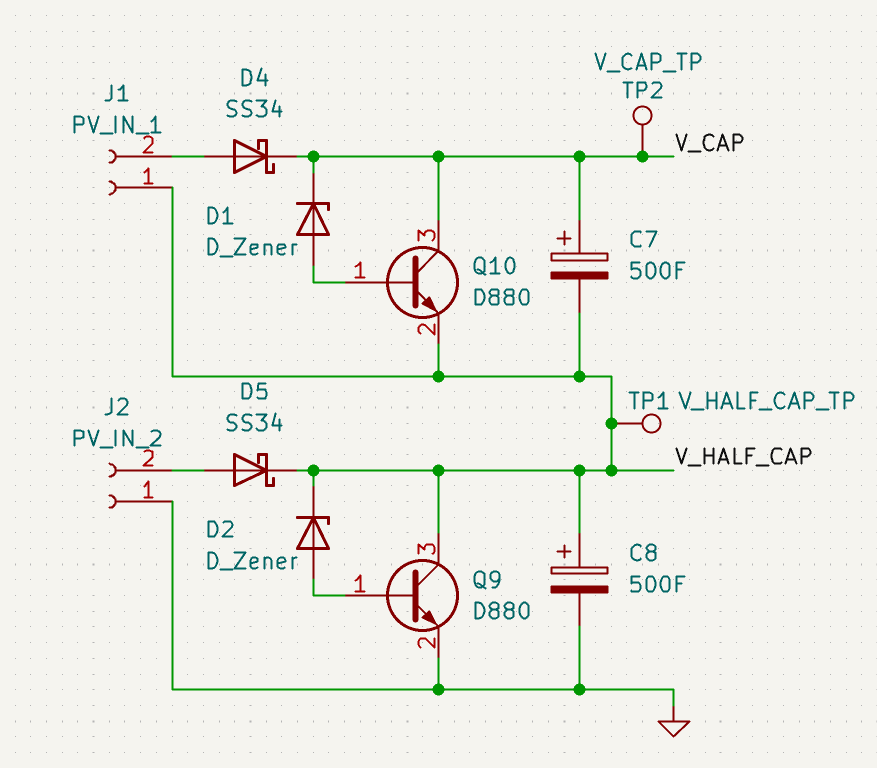
\includegraphics[width=0.9\textwidth]{fig/capacitor_charging_section_zener.png}
        \caption{Sekcja ładowania superkondesatorów z użyciem diod zenera (D1,~D2)}
        \label{rys:cond-charging-zener}
    \end{minipage}\hfill
    \begin{minipage}{0.45\textwidth}
        \centering
        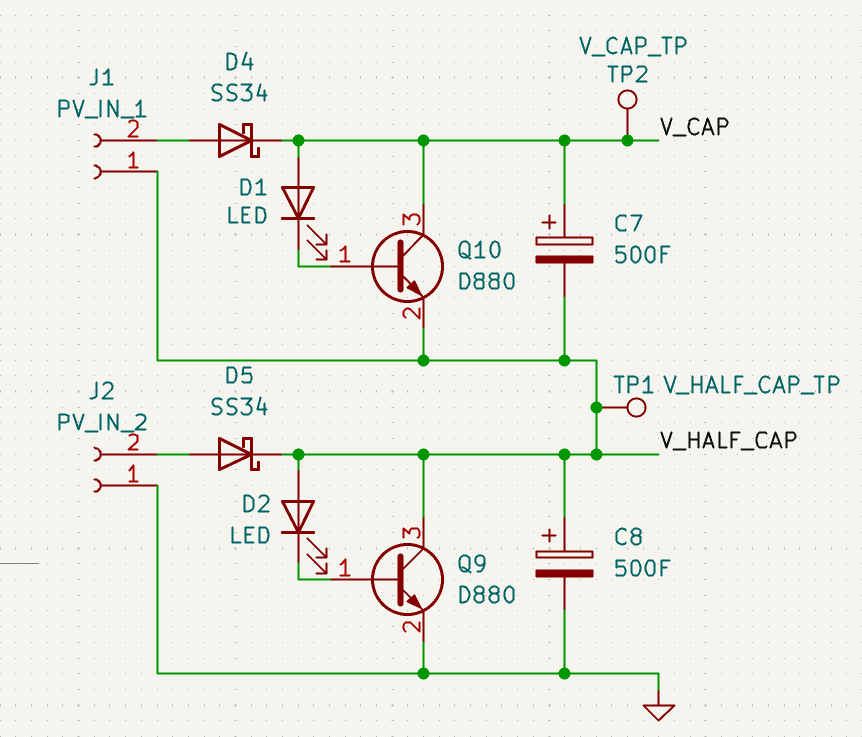
\includegraphics[width=0.9\textwidth]{fig/capacitor_charging_section_led.png}
        \caption{Sekcja ładowania superkondesatorów z użyciem diod LED (D1,~D2)}
        \label{rys:cond-charging-led}
    \end{minipage}
\end{figure}

\begin{table}[h!]
    \centering
    \begin{tabular}{|r|c|c|}
        \hline
        I\textsubscript{E} [mA] & U\textsubscript{Wy} Zener [V]& U\textsubscript{Wy} LED [V] \\
        \hline
        5   & 1,80 & 2,38 \\
        20  & 2,09 & 2,45 \\
        50  & 2,25 & 2,50 \\ 
        100 & 2,40 & 2,53 \\
        200 & 2,65 & 2,57 \\
        500 & 3,00 & 2,68 \\
        \hline
    \end{tabular}
    \caption{Napięcie wyjściowe U\textsubscript{Wy} regulatora bocznikowego przy użyciu diody Zenera i diody LED, dla prądu emitera I\textsubscript{E} tranzystora zwierającego. Do testu użyto zasilacza stałoprądowego.}
    \label{tab:zener-led-voltage-comparison}
\end{table}

\subsection{Układ regulacji napięcia}
Układ regulacji napięcia, przedstawiony na rysunku \ref*{rys:voltage_regulation}, składa się z 2 połączonych ze sobą układów. W celu wykorzystania jak największej ilości energii, zgromadzonej w superkondesatorach, napięcie jest podwyższane poprzez przetwornicę typu step-up --- zbudowaną w oparciu o układ ME210833P --- do wartości 5V. Dzięki temu połączone szeregowo superkondensatory mogą być rozładowane do napięcia mniejszego niż 1V\cite{ME2108A33P}. Podwyższone napięcie jest następnie obniżane do wartości 3.3V z użyciem regulatora liniowego HT7333 o niskim poborze mocy i niskim prądzie spoczynkowym\cite{HT7333}.


\begin{figure}[H]
    \centering
    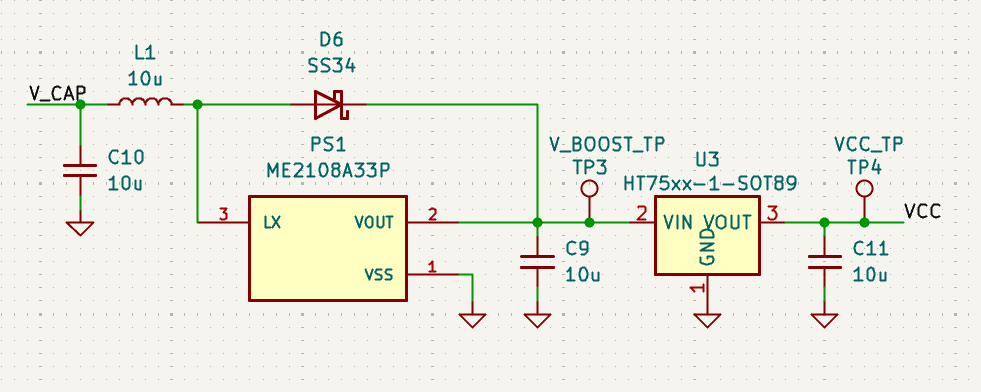
\includegraphics[width=0.9\textwidth]{fig/voltage_regulation_section.png}
    \caption{Układ regulacji napięcia oparty o przetwornicę step-up i regulator liniowy.}
    \label{rys:voltage_regulation}
\end{figure}


\subsection{Magistrala $I^2C$}
\subsection{Mikrokontroler ATmega328p}
\subsection{Układ komunikacji radiowej}

\section{Elementy pomiarowe}
\subsection{Barometr, higrometr i termometr}
\subsection{Moduł z licznikiem Geigera-Müllera}
\subsection{Moduł pomiaru nateżenia światła}

\section{Elementy dodatkowe}
\subsection{Magistrala 1-Wire}
\subsection{Wolne wyprowadzenia GPIO}

\chapter{Oprogramowanie}

\section{Język Rust w programowaniu mikrokontrolerów}

\section{Narzędzia i biblioteki}


\section{Obsługa elementów pomiarowych}
\label{section:devices_programming}
W celu ograniczenia wykorzystania zasobów pamięciowych mikrokontrolera znaczna część konfiguracji urządzeń pomiarowych realizowana jest na etapie kompilacji. Rozbudowany system typów \translation{type system} języka Rust umożliwia zwięzłe i czytelne wyrażenie konfiguracji z wykorzystaniem typów generycznych \translation{generic types}, cech \translation{traits} oraz stałych czasu kompilacji \translation{const generics}.

\subsection{Moduł AHT20 --- czujnik temperatury i wilgotności względnej}
Komunikacja z modułem AHT20 realizowana jest za pośrednictwem magistrali \isqrc poprzez wysyłanie dedykowanych komend sterujących. Moduł nie wymaga przesyłania danych konfiguracyjnych w trakcie działania. Zgodnie z notą katalogową producenta \cite{AHT20} urządzenie obsługuje następujący zestaw komend:
\begin{itemize}
    \item \textbf{Inicjalizacja} --- wymuszenie procedury kalibracji wewnętrznej układu;
    \item \textbf{Wyzwolenie pomiaru} --- zainicjowanie akwizycji danych oraz
          ich zapis do wewnętrznej pamięci urządzenia;
    \item \textbf{Odczyt statusu} --- weryfikacja stanu kalibracji układu oraz
          gotowości do przeprowadzenia kolejnego pomiaru.
\end{itemize}

Procedura inicjalizacji modułu, przedstawiona na listingu \ref*{lst:aht20_init}, rozpoczyna się od odczekania czasu rozruchu wynoszącego \SI{40}{\milli\second}, po którym następuje odczyt rejestru statusu. W przypadku braku flagi kalibracji wysyłana jest komenda inicjalizacji, a następnie wprowadzane jest opóźnienie \SI{10}{\milli\second} niezbędne do jej wykonania:

\begin{lstlisting}[language=Rust, caption={Inicjalizacja modułu AHT20}, label={lst:aht20_init}]
delay.delay_ms(40);

let status = self.read_status(i2c)?;

if status & STATUS_CALIBRATED_BIT == 0 {
    i2c.write(self.address, &COMMAND_INITIALIZE)?;
    delay.delay_ms(10);
}
\end{lstlisting}


\subsection{Moduł BMP280}


\subsection{Moduł VEML7700}


\subsection{Modułu z licznikiem Geigera-Müllera}

\section{Komunikacja radiowa}
\subsection{Serializacja danych}
\subsection{Zabezpieczenie danych}
[Nie zaimplementowane]
\subsection{Transmisja danych}

\chapter{Pomiary}
Rozdział ten ma za zadanie opisać pomiary dokonane
za pomocą czujnika klimatycznego realizowanego
w~tym projekcie.

\section{Przygotowanie do pomiarów}
Dla wygody użytkowania czujnik oraz kondensatory zostały 
zamontowane na ramie stworzonej w~technologii druku 3D,
widocznej na rysunku~\ref{rys:frame}.
Rysunek~\ref{rys:pcb_on_frame} przedstawia płytkę drukowaną 
przymocowaną do ramy,
uzupełnioną o~moduły pomiarowe, nadajnik radiowy oraz
diodę statusu. Dioda została podpięta do linii zasilania
nieużywanej magistrali 1--Wire.

\begin{figure}[H]
    \centering
    \begin{minipage}{0.45\textwidth}
        \centering
        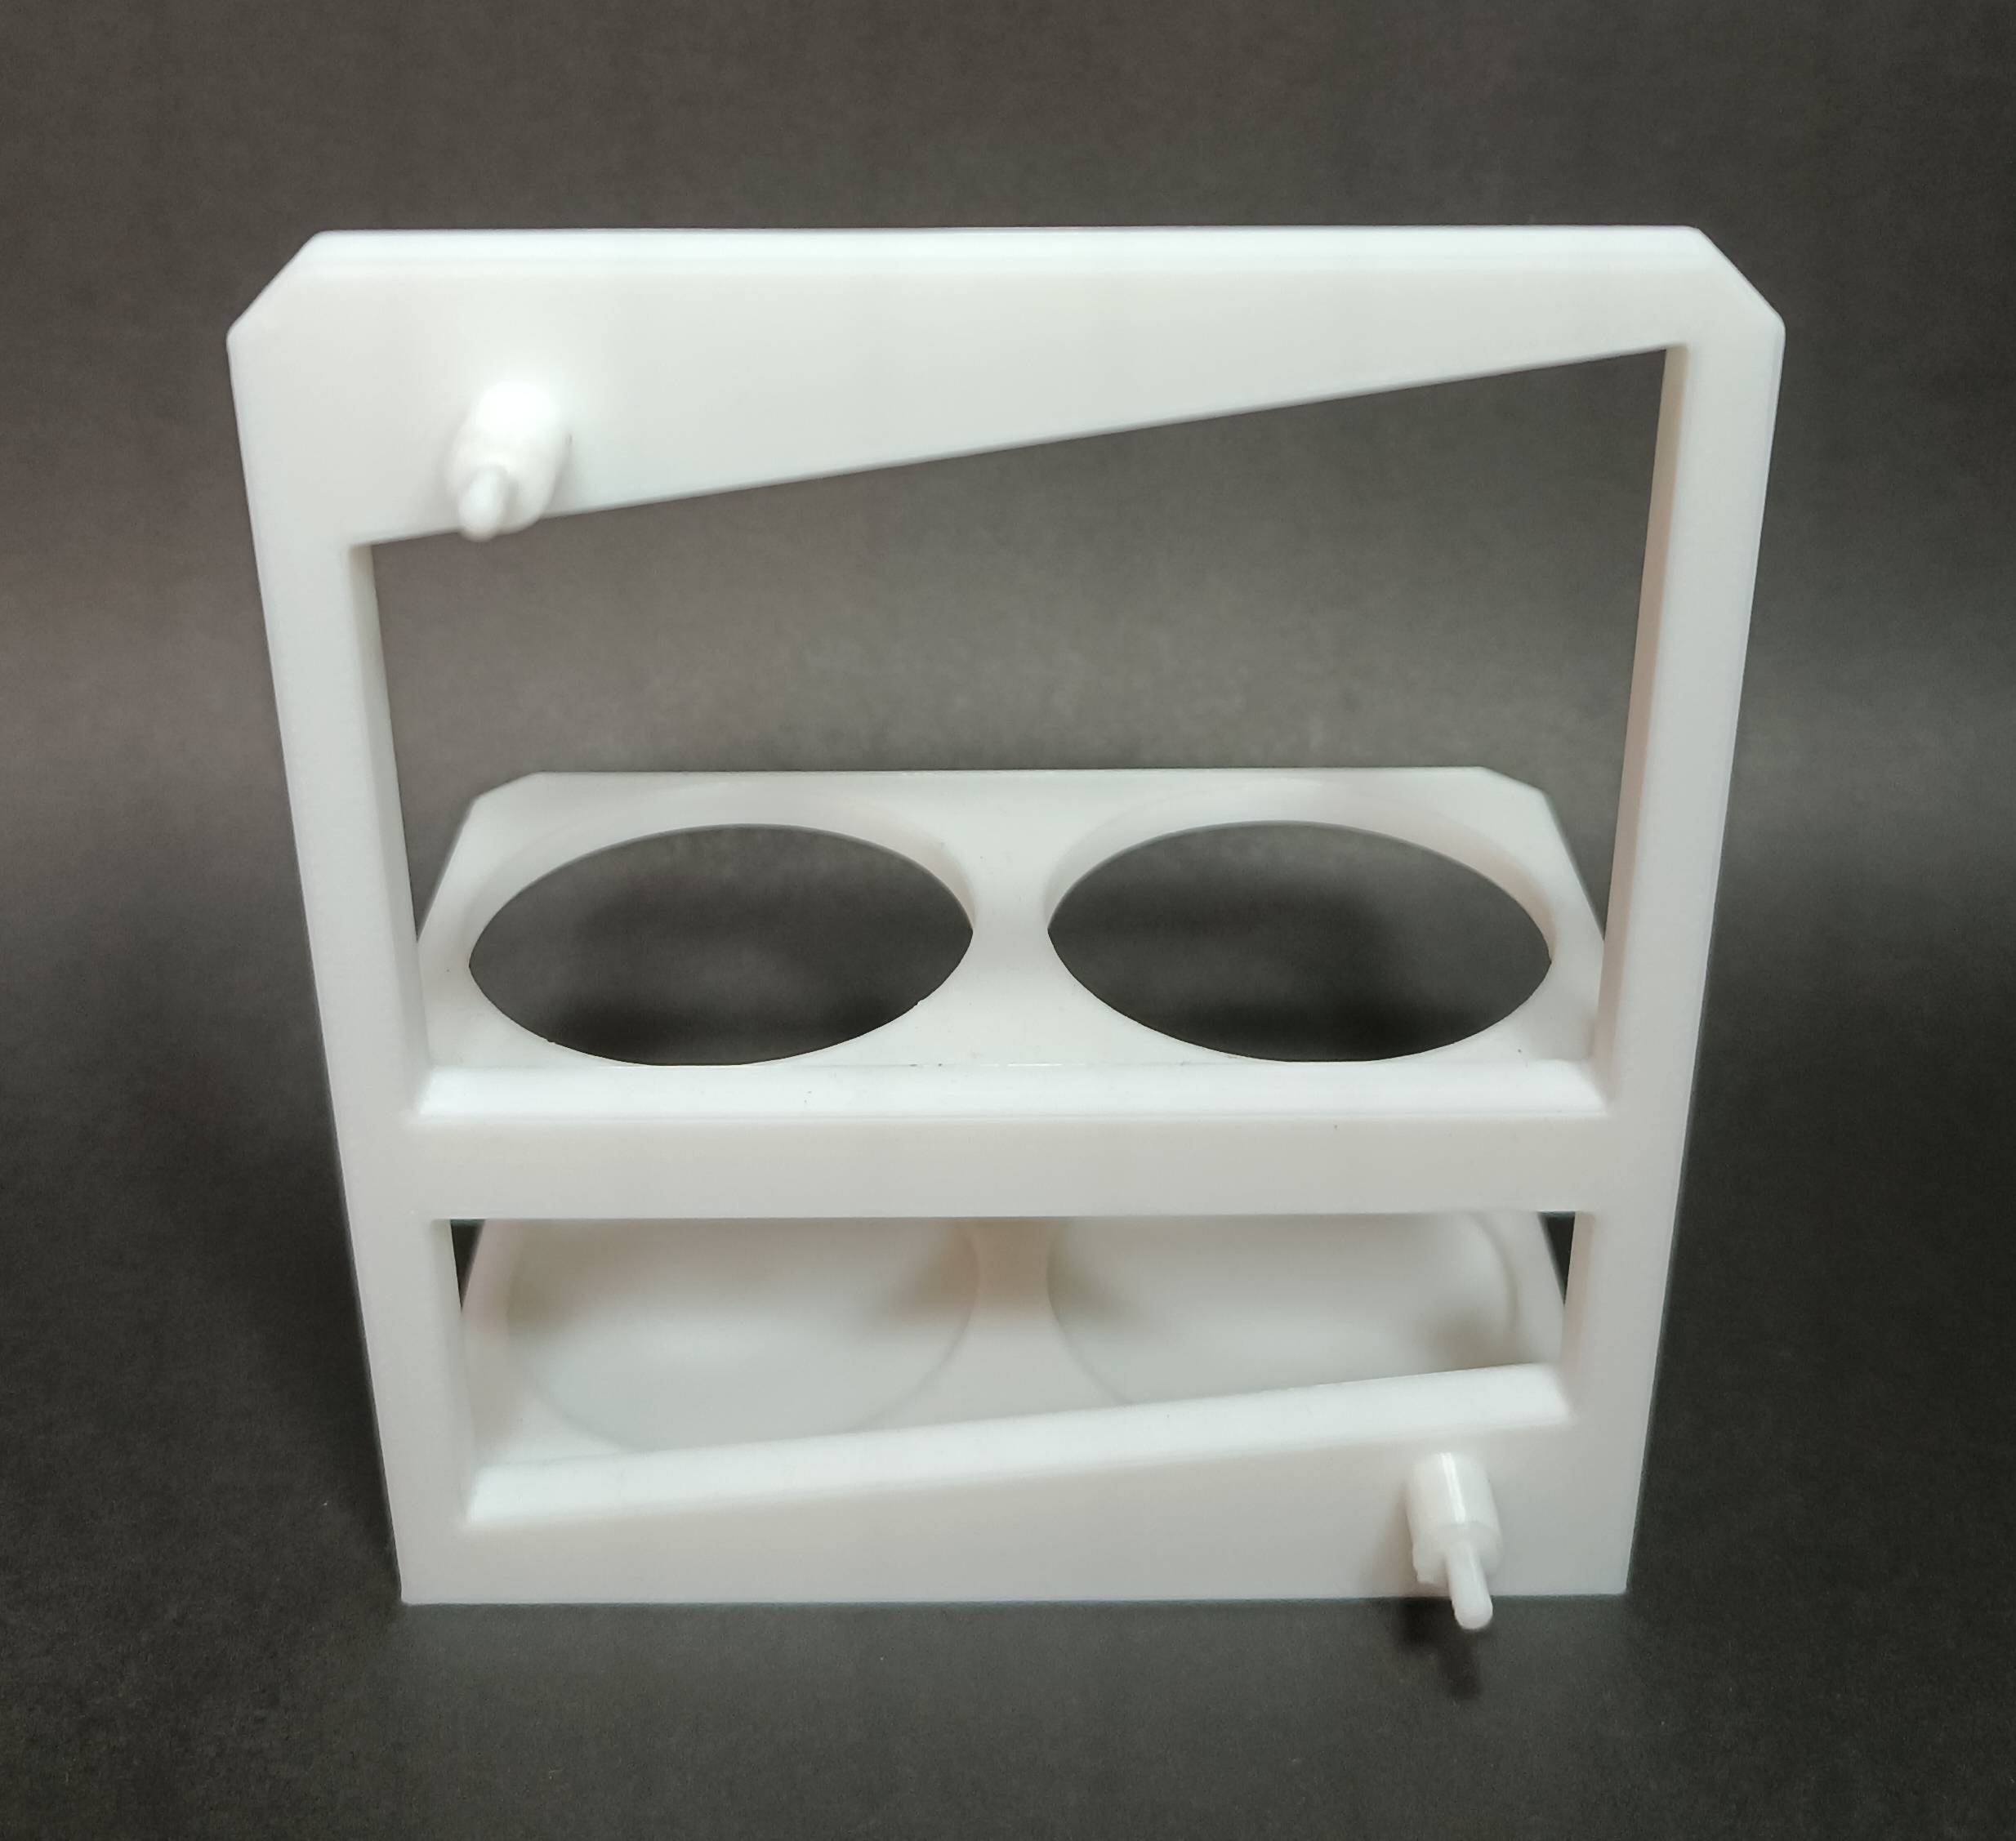
\includegraphics[width=0.9\textwidth]{fig/img/frame_front.png}
    \end{minipage}\hfill
    \begin{minipage}{0.45\textwidth}
        \centering
        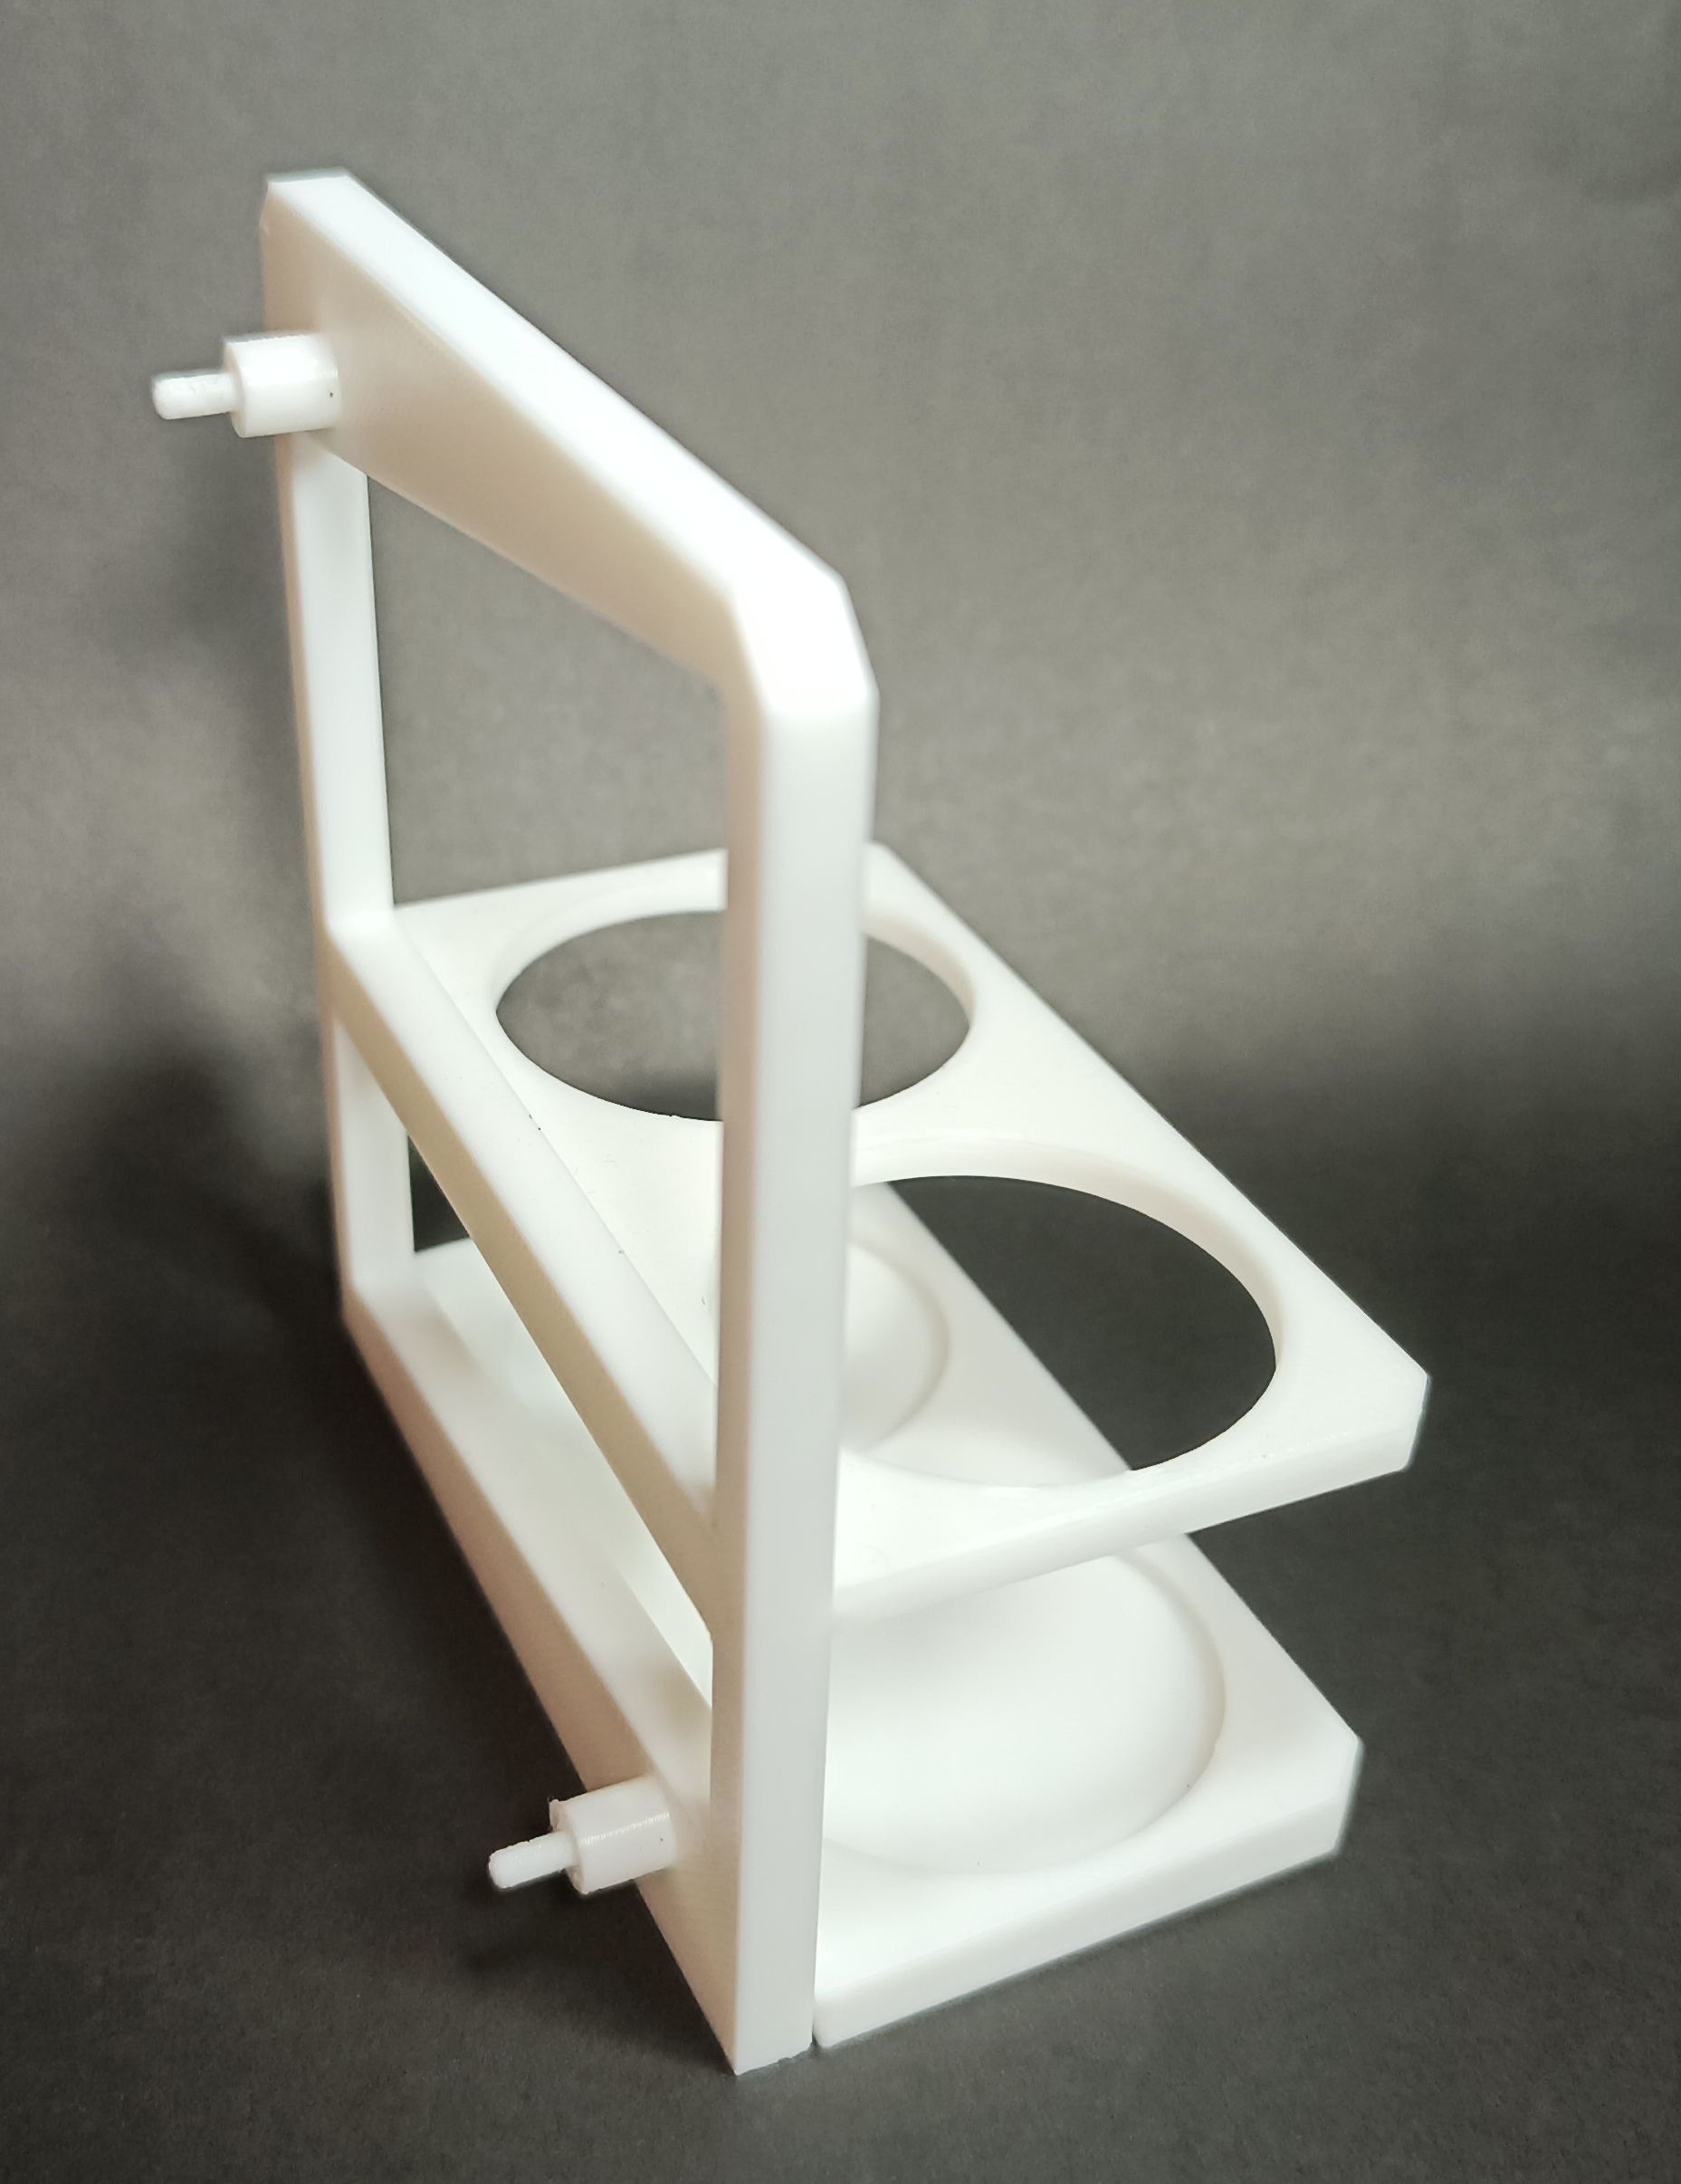
\includegraphics[width=0.9\textwidth]{fig/img/frame_side.png}
    \end{minipage}
    \caption{Rama służąca do podtrzymania płytki drukowanej 
    i~superkondensatorów}
    \label{rys:frame}
\end{figure}

\begin{figure}[H]
    \centering
    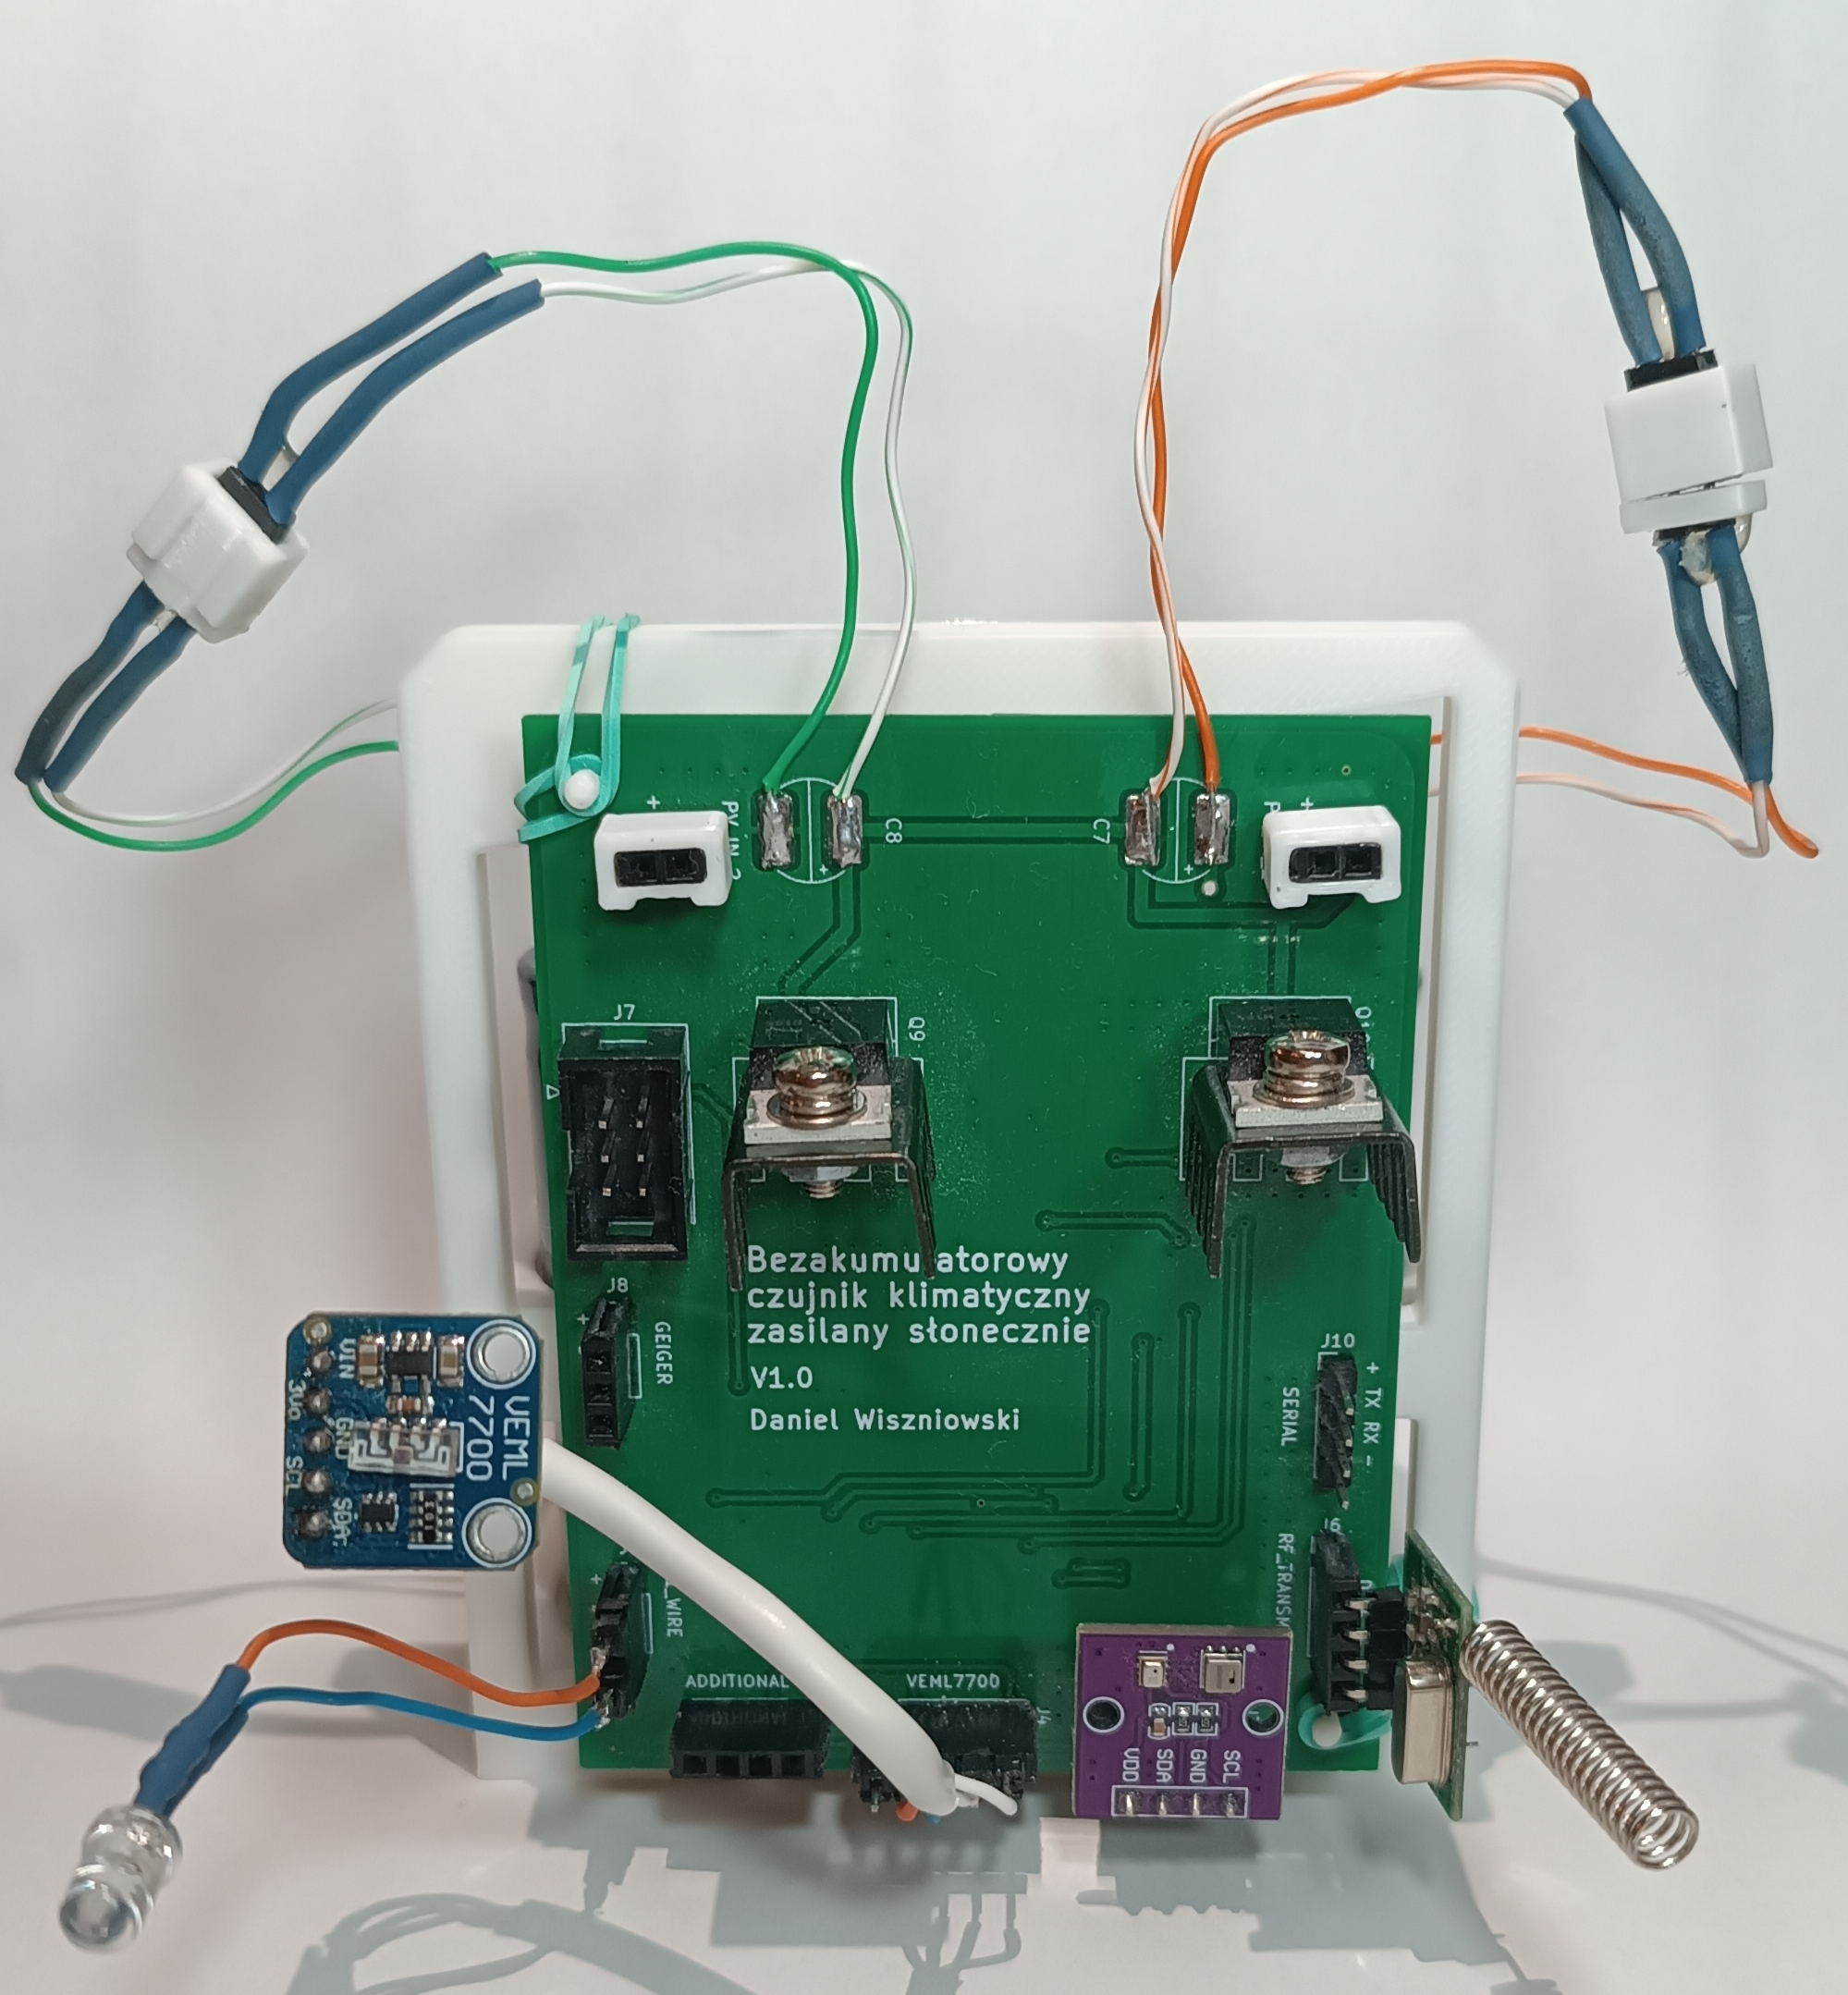
\includegraphics[width=0.9\textwidth]{fig/img/full_test_setup.png}
    \caption{Płytka drukowana uzupełniona o~moduły pomiarowe, nadajnik 
    radiowy oraz diodę statusu umieszczona na ramie i~podłączona do 
    superkondensatorów}
    \label{rys:pcb_on_frame}
\end{figure}

Układ został uzupełniony o~2 monokrystaliczne panele 
fotowoltaiczne. Rysunek~\ref{rys:pv_panel} przedstawia jeden 
z~tych paneli.

\begin{figure}[H]
    \centering
    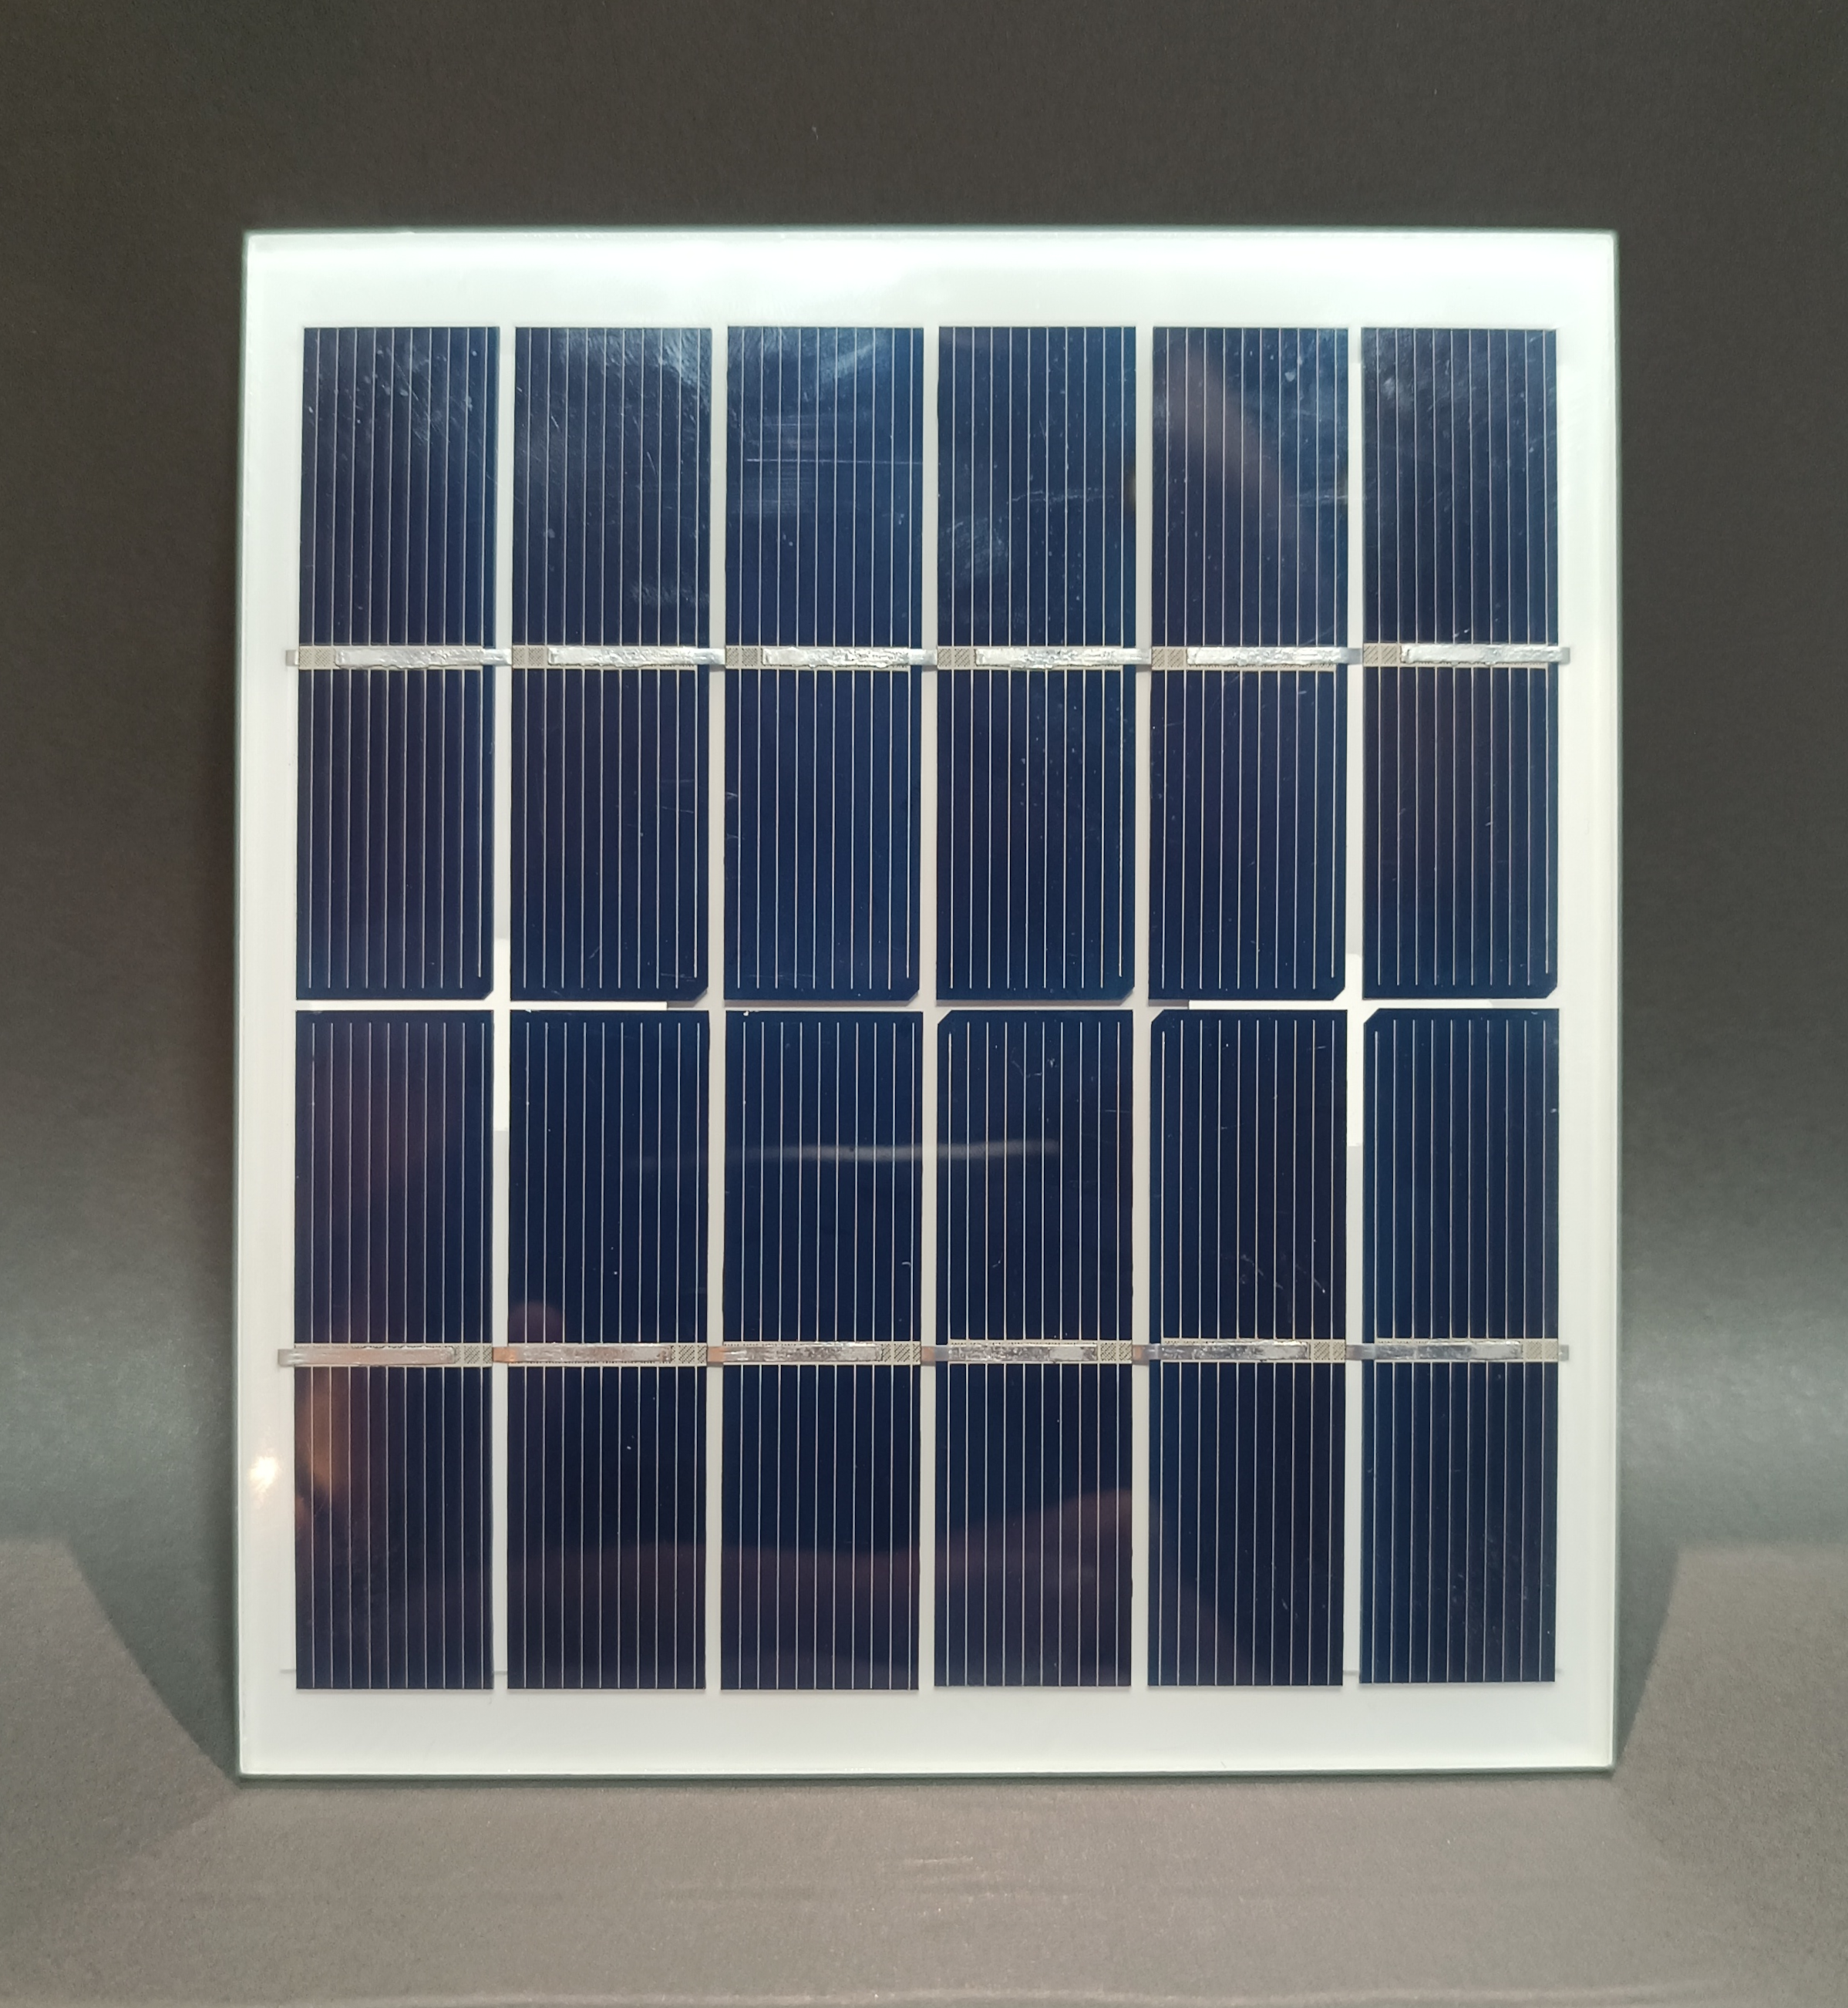
\includegraphics[width=0.9\textwidth]{fig/img/pv_panel.png}
    \caption{Monokrystaliczny panel fotowoltaiczny użyty do zasilenia czujnika
    klimatycznego}
    \label{rys:pv_panel}
\end{figure}

Do odbioru i~przetwarzania danych wysyłanych przez czujnik
klimatyczny wykorzystano odbiornik obsługujący częstotliwość 
\SI{433}{\mega\hertz} podłączony do płytki Arduino NANO.
Arduino NANO przy pomocy autorskiej biblioteki
\texttt{ook\_433mhz} umożliwiało dekodowanie danych odebranych 
od czujnika, a~następnie wysyłanie ich przez port szeregowy 
do komputera, który gromadził je w~pliku CSV.


\section{Przebieg pomiarów}
W~celu przetestowania czujnika klimatycznego w~warunkach
wewnętrznych jak i~zewnętrznych został on poddany
testom trwającym odpowiednio \SI{10}{\hour} i~\SI{31}{\hour},
w~których czujnik wysyłał dane w~jednominutowych
odstępach. Podczas obydwu testów mierzona była 
temperatura, wilgotność względna, ciśnienie atmosferyczne
oraz napięcie na okładkach kondensatorów zasilających.

\subsection*{Pomiary wewnętrzne}
Czujnik funkcjonował poprawnie w~trakcie 10-godzinnego
testu w~warunkach wewnętrznych, trwającego od godziny 
23:58 do godziny 10:42. 
Uzyskane dane pomiarowe to: 
temperatura (rysunek~\ref{rys:graph_temp_ins}),
wilgotność względna (rysunek~\ref{rys:graph_hum_ins}),
ciśnienie atmosferyczne (rysunek~\ref{rys:graph_press_ins}),
natężenie światła (rysunek~\ref{rys:graph_lux_ins})
oraz napięcie na kondensatorach (rysunek~\ref{rys:graph_volt_ins}).

W~celu wykonania tego testu czujnik klimatyczny został 
umieszczony z~dala od źródeł ciepła i~światła. Panele
fotowoltaiczne również były umieszczone w~dużej odległości
od bezpośredniego światła słonecznego.

\begin{figure}[H]
    \centering
    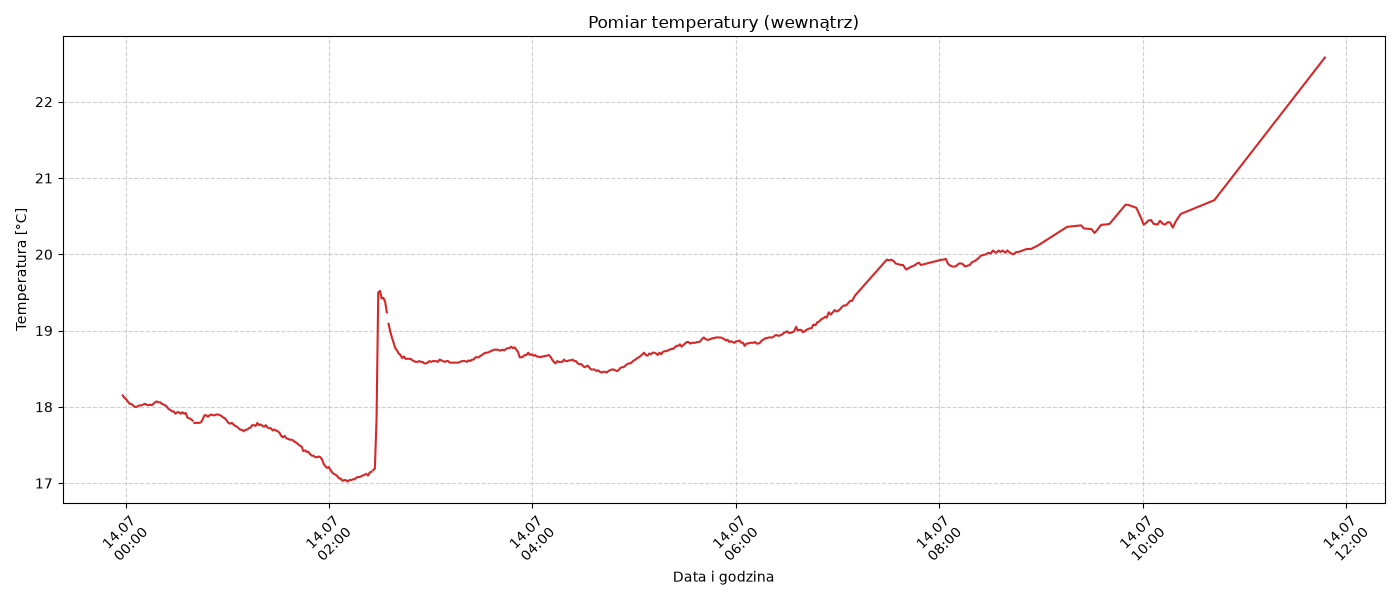
\includegraphics[width=0.9\textwidth]{fig/graphs/temperatura_inside.png}
    \caption{Wykres przedstawiający pomiary wartości temperatury w~warunkach wewnętrznych}
    \label{rys:graph_temp_ins}
\end{figure}

\begin{figure}[H]
    \centering
    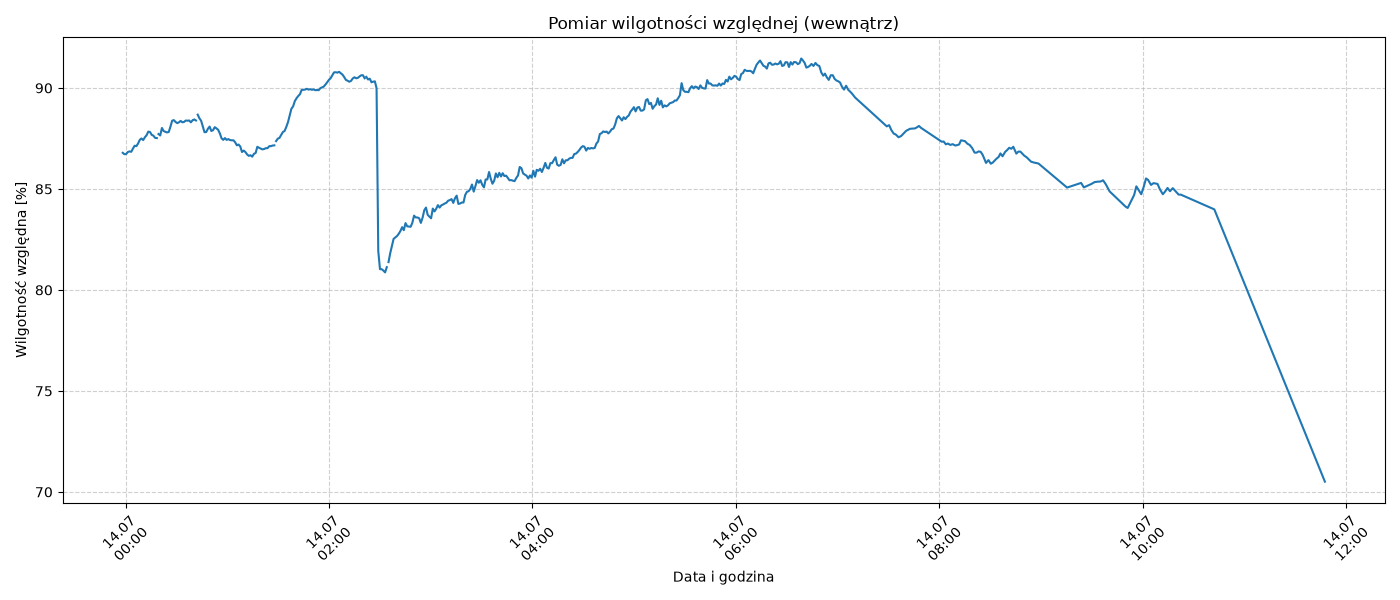
\includegraphics[width=0.9\textwidth]{fig/graphs/humidity_inside.png}
    \caption{Wykres przedstawiający pomiary wartości wilgotności względnej w~warunkach wewnętrznych}
    \label{rys:graph_hum_ins}
\end{figure}

\begin{figure}[H]
    \centering
    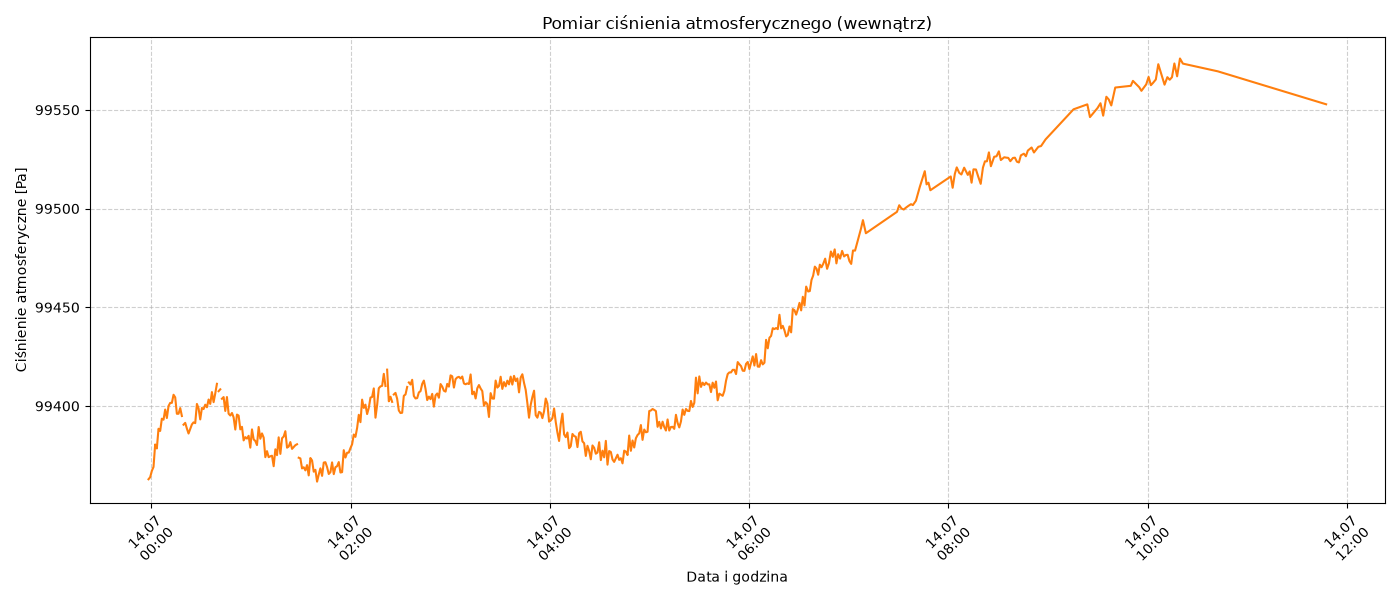
\includegraphics[width=0.9\textwidth]{fig/graphs/pressure_inside.png}
    \caption{Wykres przedstawiający pomiary wartości ciśnienia atmosferycznego w~warunkach wewnętrznych}
    \label{rys:graph_press_ins}
\end{figure}

\begin{figure}[H]
    \centering
    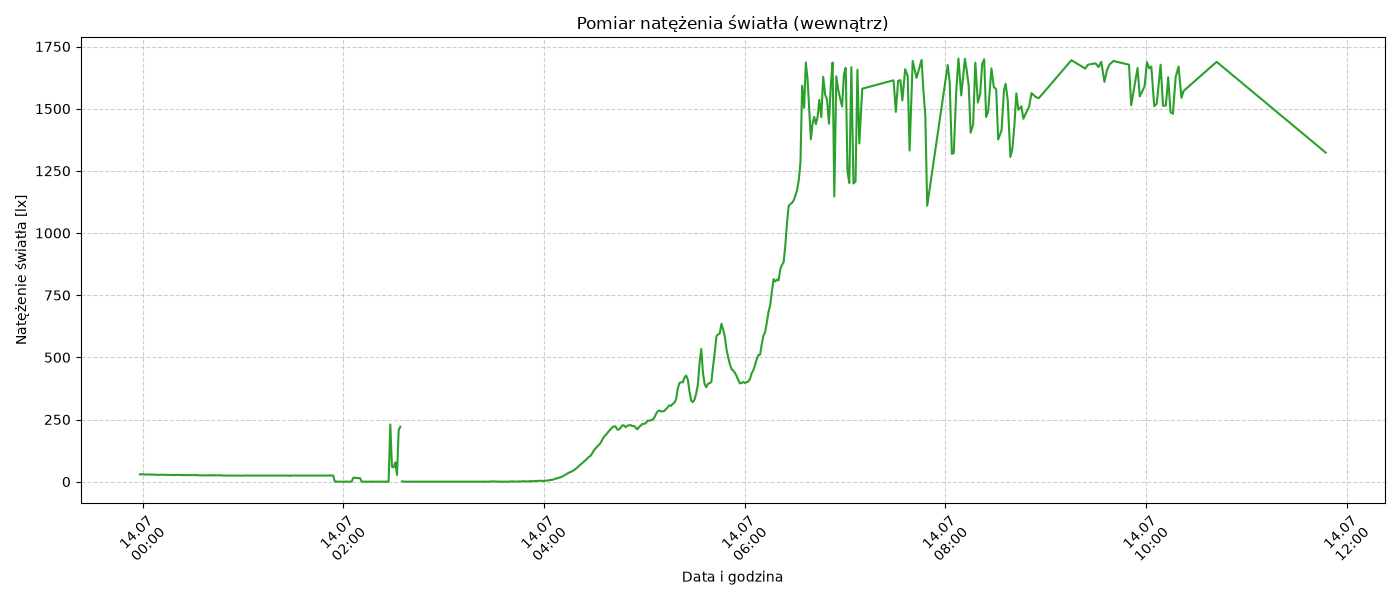
\includegraphics[width=0.9\textwidth]{fig/graphs/lux_inside.png}
    \caption{Wykres przedstawiający pomiary wartości natężenie światła w~warunkach wewnętrznych}
    \label{rys:graph_lux_ins}
\end{figure}

\begin{figure}[H]
    \centering
    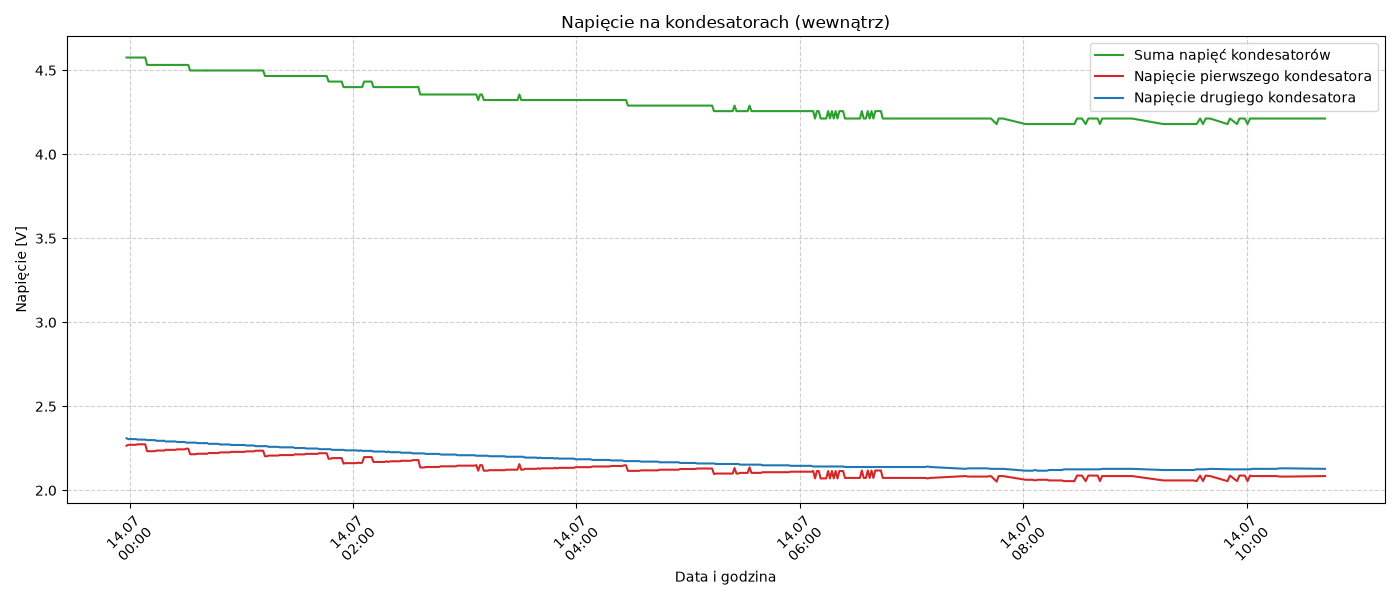
\includegraphics[width=0.9\textwidth]{fig/graphs/voltage_inside.png}
    \caption{Wykres przedstawiający pomiary wartości napięcia na okładkach kondensatorów w~warunkach wewnętrznych}
    \label{rys:graph_volt_ins}
\end{figure}


\subsection*{Pomiary zewnętrzne}
Podobnie, jak w~przypadku pomiarów wewnętrznych, nie 
odnotowano zakłóceń w~pracy czujnika klimatycznego. Test trwał
od godziny 15:28 dnia 14 lipca, do godziny 22:25 dnia 
następnego. Zebrane w~tym czasie dane zostały przedstawione
na wykresach: 
temperatury (rysunek~\ref{rys:graph_temp}),
wilgotności względnej (rysunek~\ref{rys:graph_hum}),
ciśnienia atmosferycznego (rysunek~\ref{rys:graph_press}),
natężenia światła (rysunek~\ref{rys:graph_lux})
oraz napięcia na kondensatorach (rysunek~\ref{rys:graph_volt}).

Do przeprowadzenia tego testu czujnik klimatyczny (jak i~panele 
fotowoltaiczne) znajdował się w~cieniu, na skierowanej na 
południowy zachód ścianie domu. Taka lokalizacja nie zapewniała
optymalnych warunków nasłonecznienia paneli fotowoltaicznych.

\begin{figure}[H]
    \centering
    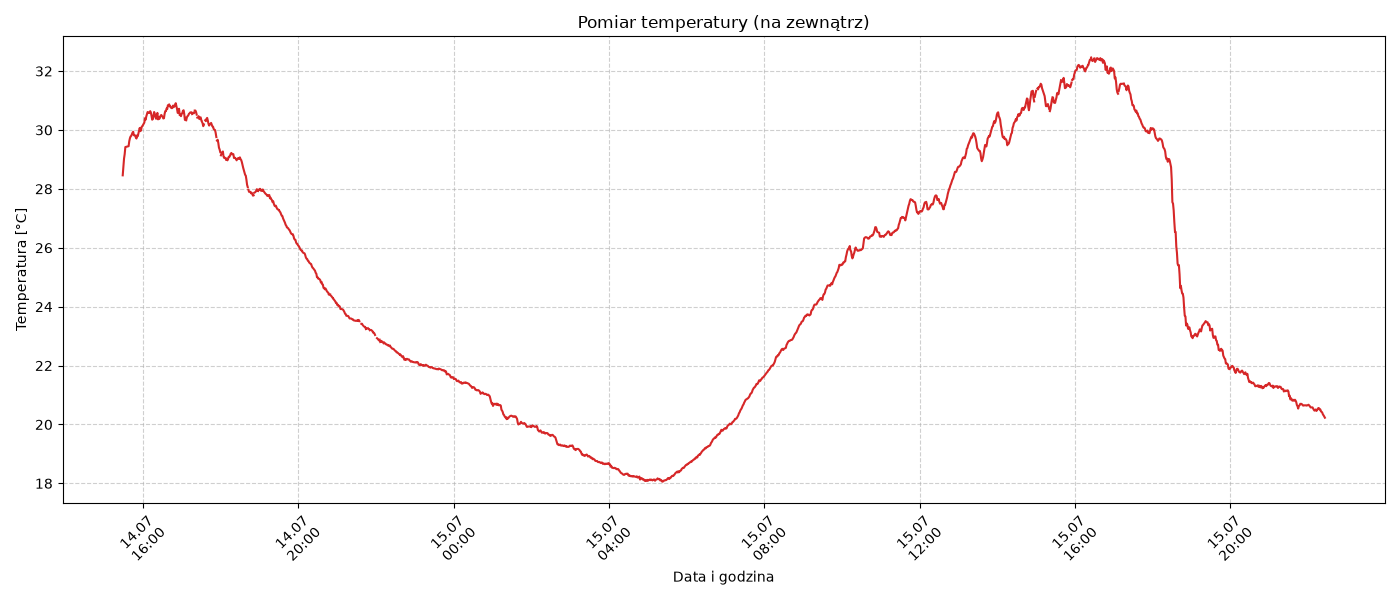
\includegraphics[width=0.9\textwidth]{fig/graphs/temperatura.png}
    \caption{Wykres przedstawiający pomiary wartości temperatury w~warunkach zewnętrznych}
    \label{rys:graph_temp}
\end{figure}

\begin{figure}[H]
    \centering
    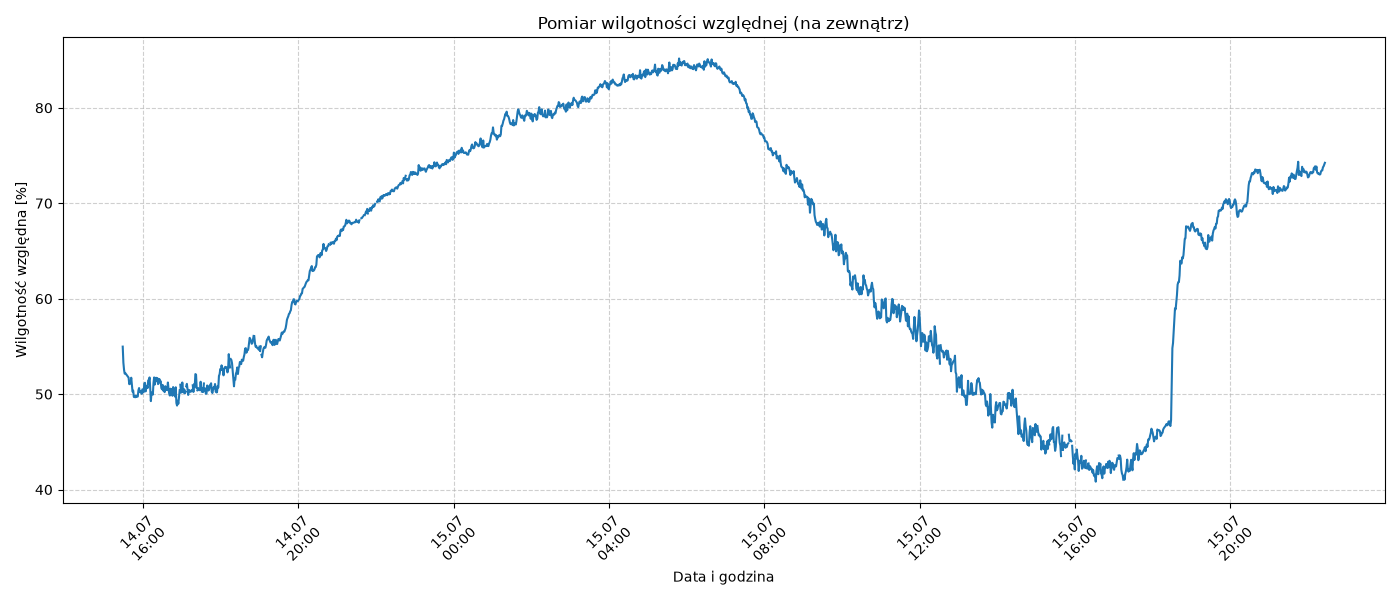
\includegraphics[width=0.9\textwidth]{fig/graphs/humidity.png}
    \caption{Wykres przedstawiający pomiary wartości wilgotności względnej w~warunkach zewnętrznych}
    \label{rys:graph_hum}
\end{figure}

\begin{figure}[H]
    \centering
    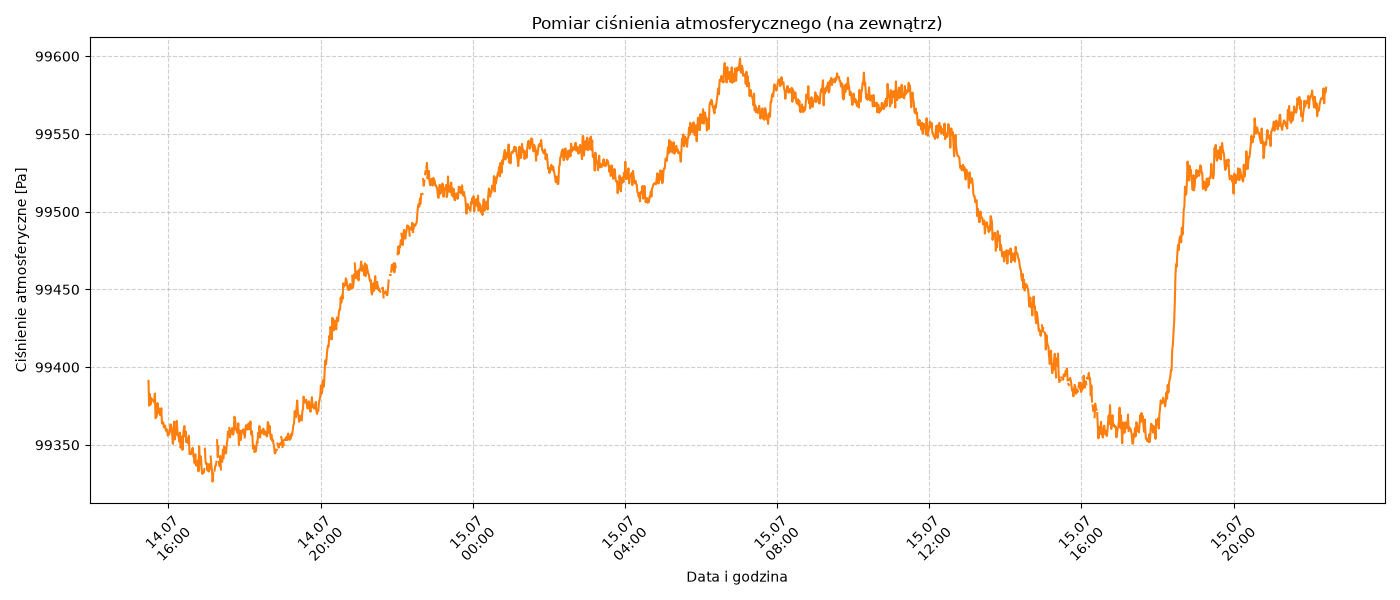
\includegraphics[width=0.9\textwidth]{fig/graphs/pressure.png}
    \caption{Wykres przedstawiający pomiary wartości ciśnienia atmosferycznego w~warunkach zewnętrznych}
    \label{rys:graph_press}
\end{figure}

\begin{figure}[H]
    \centering
    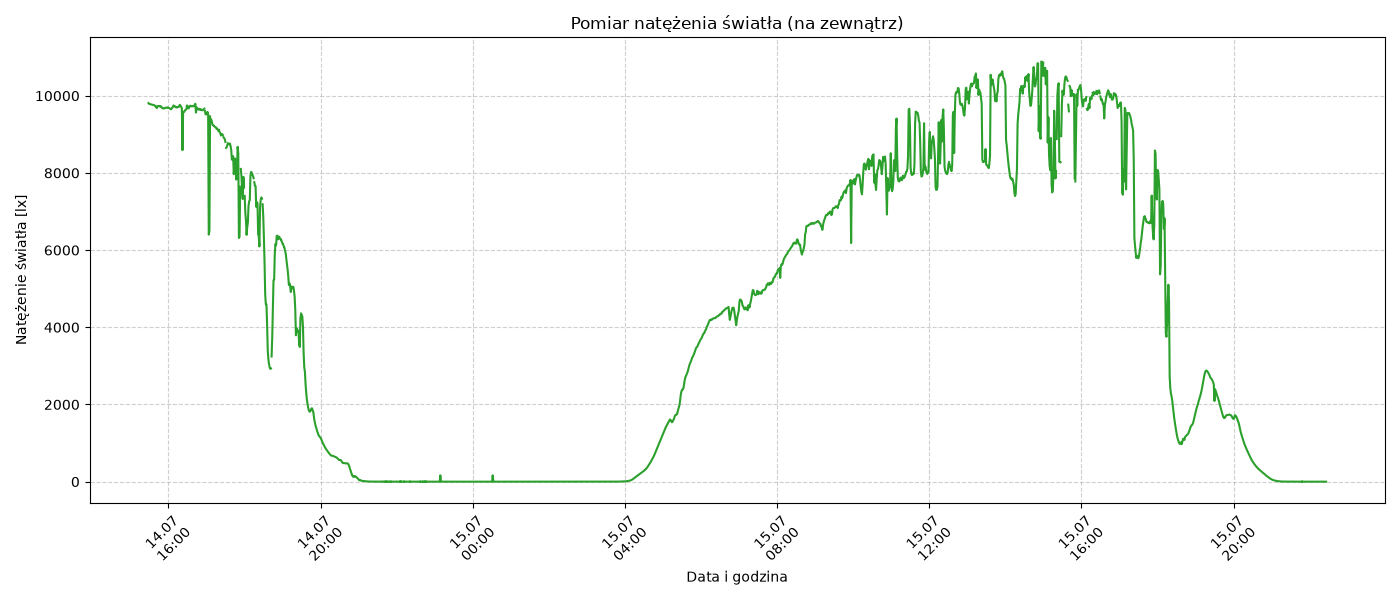
\includegraphics[width=0.9\textwidth]{fig/graphs/lux.png}
    \caption{Wykres przedstawiający pomiary wartości natężenie światła w~warunkach zewnętrznych}
    \label{rys:graph_lux}
\end{figure}

\begin{figure}[H]
    \centering
    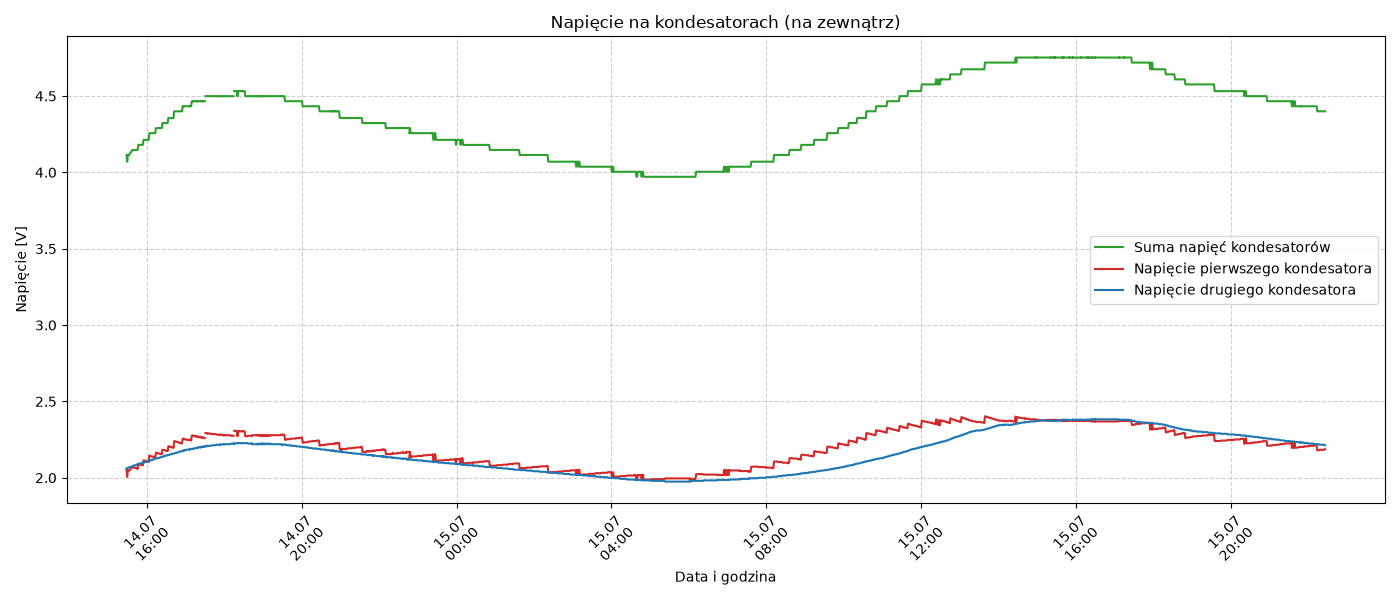
\includegraphics[width=0.9\textwidth]{fig/graphs/voltage.png}
    \caption{Wykres przedstawiający pomiary wartości napięcia na okładkach kondensatorów w~warunkach zewnętrznych}
    \label{rys:graph_volt}
\end{figure}


\section{Wnioski}
Utworzony na potrzeby tego projektu czujnik klimatyczny 
może być stosowany zarówno w~warunkach wewnętrznych, 
jak i~zewnętrznych. 

W~przypadku użycia czujnika na zewnątrz panele fotowoltaiczne 
umożliwiają naładowanie superkondensatorów w~ciągu dnia, nawet przy 
braku bezpośrednio padającego na nie światła słonecznego.
Natomiast w~przypadku użycia wewnętrznego koniecznym może być
ustawienie paneli bliżej bezpośredniego źródła światła słonecznego. 

Zgromadzony w~superkondensatorach ładunek pozwala na 
podtrzymanie pracy urządzenia przez okres 12 godzin, 
rozładowując się w~tym czasie do sumarycznej wartości 
\SI{4}{\volt}, pozostawiając~\SI{3}{\volt} zapasu.

\chapter*{Podsumowanie} % jak we wstępie
\addcontentsline{toc}{chapter}{Podsumowanie}
\chaptermark{Podsumowanie}

W ramach niniejszej pracy zaprojektowano i~wykonano funkcjonalny prototyp
bezakumulatorowego czujnika klimatycznego, zasilanego wyłącznie energią
pochodzącą z~paneli fotowoltaicznych i~magazynowaną w~superkondensatorach.
Zrealizowane urządzenie dokonuje pomiaru temperatury, wilgotności
względnej, ciśnienia atmosferycznego, natężenia oświetlenia oraz poziomu
promieniowania jonizującego, a~zebrane dane przesyła bezprzewodowo, za
pomocą autorskiej biblioteki \texttt{ook\_433mhz}, do stacji bazowej.
Przeprowadzone testy, trwające odpowiednio 10 i~31 godzin w~warunkach
wewnętrznych oraz zewnętrznych, potwierdziły poprawność działania
zbudowanego układu, a~ładunek zgromadzony w~superkondensatorach pozwolił
na podtrzymanie pracy urządzenia bez dostępu do źródła zasilania przez
okres około 12 godzin.
 
Wybór języka Rust do implementacji oprogramowania sterującego
mikrokontrolerem okazał się uzasadniony --- statyczna weryfikacja
poprawności typów na etapie kompilacji pozwoliła na wyeliminowanie części
błędów już na etapie tworzenia kodu, bez narzutu czasu wykonania. Należy
jednak zaznaczyć, że część mechanizmów języka, takich jak arytmetyka
liczb 64-bitowych, nie jest natywnie wspierana przez architekturę AVR
i~wymaga emulacji programowej, co negatywnie wpływa na wydajność kodu.
 
Zrealizowany projekt można rozwijać w~kilku kierunkach, między innymi
poprzez wykorzystanie przewidzianej na płytce magistrali 1-Wire do
podłączenia dodatkowych czujników, wprowadzenie mechanizmu potwierdzeń
w~jednokierunkowym obecnie protokole radiowym oraz przeprowadzenie
długoterminowych testów sezonowych. Podsumowując, cel pracy ---
zaprojektowanie i~wykonanie autonomicznego, bezobsługowego czujnika
klimatycznego niewymagającego akumulatora --- został osiągnięty, a~samo
urządzenie potwierdza, że superkondensatory w~połączeniu z~zasilaniem
fotowoltaicznym stanowią realną alternatywę dla bateryjnych stacji
pogodowych
 % jeśli są listingi:
\cleardoublepage
\phantomsection
\addcontentsline{toc}{chapter}{Spis listingów}
\renewcommand{\lstlistlistingname}{Spis listingów}
\lstlistoflistings{}

 % jeśli są tabele:
\cleardoublepage
\phantomsection
\addcontentsline{toc}{chapter}{Spis tabel}
\listoftables{}

 % jeśli są rysunki:
\cleardoublepage
\phantomsection
\addcontentsline{toc}{chapter}{Spis rysunków}
\listoffigures{}

\cleardoublepage
\phantomsection
\addcontentsline{toc}{chapter}{Bibliografia} % też ręczne dodanie do spisu treści, jak Wstęp
\label{sec:bibliografia}
\bibliography{ref.bib}

\end{document}
